\chapter{Clase 1: Introducción a la regresión lineal}

\section{Motivación: explicar y predecir}

En muchos estudios interesa describir cómo cambia una característica de interés en relación con otras variables. Por ejemplo, estudiantes, familias y universidades pueden preguntarse si es posible anticipar el promedio académico (GPA) al terminar el primer año universitario, usando información disponible antes del ingreso.

Para hacer una predicción podrían considerarse variables como el puesto del estudiante en su grupo de secundaria, el nivel general de su colegio, sus calificaciones previas y el resultado de una prueba de admisión. Estas variables no determinan el resultado de manera exacta; aportan información que puede ayudar a describir su comportamiento promedio.

\begin{figure}[H]
\centering
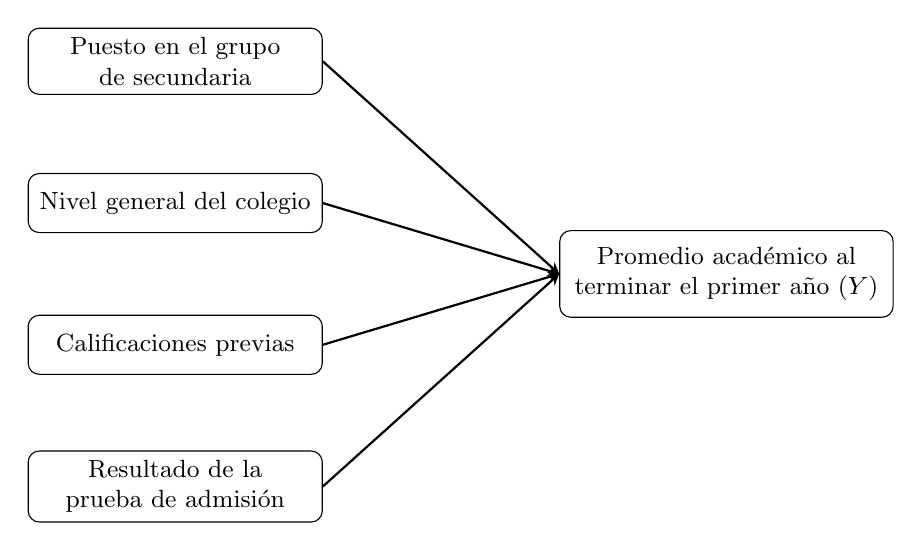
\begin{tikzpicture}[
    predictor/.style={draw,rounded corners,align=center,text width=3.5cm,minimum height=0.75cm,font=\small},
    response/.style={draw,rounded corners,align=center,text width=4.0cm,minimum height=1.1cm,font=\small},
    link/.style={->,>=stealth,thick}
]
\node[predictor] (x1) at (0,2.7) {Puesto en el grupo de secundaria};
\node[predictor] (x2) at (0,0.9) {Nivel general del colegio};
\node[predictor] (x3) at (0,-0.9) {Calificaciones previas};
\node[predictor] (x4) at (0,-2.7) {Resultado de la prueba de admisión};
\node[response] (y) at (7,0) {Promedio académico al terminar el primer año ($Y$)};
\draw[link] (x1.east) -- (y.west);
\draw[link] (x2.east) -- (y.west);
\draw[link] (x3.east) -- (y.west);
\draw[link] (x4.east) -- (y.west);
\end{tikzpicture}
\caption{Esquema de algunas variables que podrían usarse para anticipar el promedio académico.}
\label{fig:predictores-gpa}
\end{figure}

La pregunta general es cómo resumir la relación entre una variable de interés y la información disponible, y qué tan útil resulta esa relación para predecir. Los modelos de regresión ofrecen un marco para estudiar estas preguntas.

\section{Variable respuesta y variables predictoras}

Llamaremos $Y$ a la \textbf{variable respuesta} o dependiente, cuyo comportamiento queremos describir o predecir. Las variables $X_1,\ldots,X_m$ se denominan \textbf{predictoras} o independientes en el sentido del modelo: son la información que se utiliza para estudiar la respuesta. Esta denominación señala el papel de las variables dentro del modelo; no implica independencia probabilística. En esta introducción consideraremos variables cuantitativas.

El análisis de regresión se centra en describir el tipo de relación entre las variables y en usar los valores de las predictoras para estimar el valor medio esperado de $Y$. La notación
\[
\mathbb{E}(Y\mid X_1=x_1,\ldots,X_m=x_m)
\]
representa ese promedio de la respuesta para valores determinados de las predictoras.

Cuando se utiliza una relación lineal, las formas generales se escriben así:
\begin{align*}
\text{Regresión lineal simple:}\qquad
\mathbb{E}(Y\mid X=x)&=\beta_0+\beta_1x,\\
\text{Regresión lineal múltiple:}\qquad
\mathbb{E}(Y\mid X_1=x_1,\ldots,X_m=x_m)&=\beta_0+\beta_1x_1+\cdots+\beta_mx_m.
\end{align*}
La regresión es \textbf{simple} cuando se considera una sola variable predictora y \textbf{múltiple} cuando se consideran varias. En esta clase, las expresiones solo presentan la estructura de los modelos; todavía no se estiman sus parámetros ni se evalúa su precisión.

\section{Preguntas iniciales sobre la relación entre variables}

Cuando se estudian dos variables cuantitativas, conviene plantear algunas preguntas antes de construir un modelo:

\begin{enumerate}
    \item ¿Hay evidencia de que las variables estén relacionadas, o su comportamiento parece independiente?
    \item Si hay relación, ¿qué forma tiene y qué tan marcada parece?
    \item ¿Es posible predecir la variable respuesta a partir de la predictora? ¿Con qué precisión?
\end{enumerate}

El análisis de correlación describe si existe asociación entre variables y su grado. El análisis de regresión estudia la forma de la relación y plantea cómo predecir una variable respuesta a partir de una o más predictoras. En los temas siguientes del curso se estudiarán con detalle distintas herramientas para responder estas preguntas.

\section{Regresión simple: un ejemplo con calificaciones}

Para ilustrar el caso simple, consideremos los datos de diez estudiantes de primer año de universidad que aparecen en el documento de referencia. Para cada estudiante se registró la calificación de un examen de Matemáticas y los puntos finales obtenidos en Cálculo. Definimos:
\begin{itemize}
    \item $X$: calificación del examen de Matemáticas;
    \item $Y$: puntos finales en Cálculo.
\end{itemize}

Cada estudiante aporta un par de observaciones $(x_i,y_i)$, pues ambas calificaciones corresponden a la misma persona.

\begin{table}[H]
\centering
\small
\renewcommand{\arraystretch}{1.15}
\begin{tabular}{|r|r|r|r|}
\hline
\multicolumn{2}{|c|}{\textbf{Estudiantes 1--5}} & \multicolumn{2}{c|}{\textbf{Estudiantes 6--10}} \\ \hline
\textbf{$X$: Matemáticas} & \textbf{$Y$: Cálculo} & \textbf{$X$: Matemáticas} & \textbf{$Y$: Cálculo} \\ \hline
39 & 65 & 47 & 89 \\ \hline
43 & 78 & 28 & 73 \\ \hline
21 & 52 & 75 & 98 \\ \hline
64 & 82 & 34 & 56 \\ \hline
57 & 92 & 52 & 75 \\ \hline
\end{tabular}
\caption{Calificaciones de Matemáticas y puntos finales en Cálculo de diez estudiantes.}
\label{tab:calificaciones-regresion}
\end{table}

Una manera inicial de observar la relación es representar los pares en un diagrama de dispersión. Cada punto del gráfico corresponde a un estudiante; su posición horizontal indica la calificación de Matemáticas y su posición vertical los puntos de Cálculo.

\begin{figure}[H]
\centering
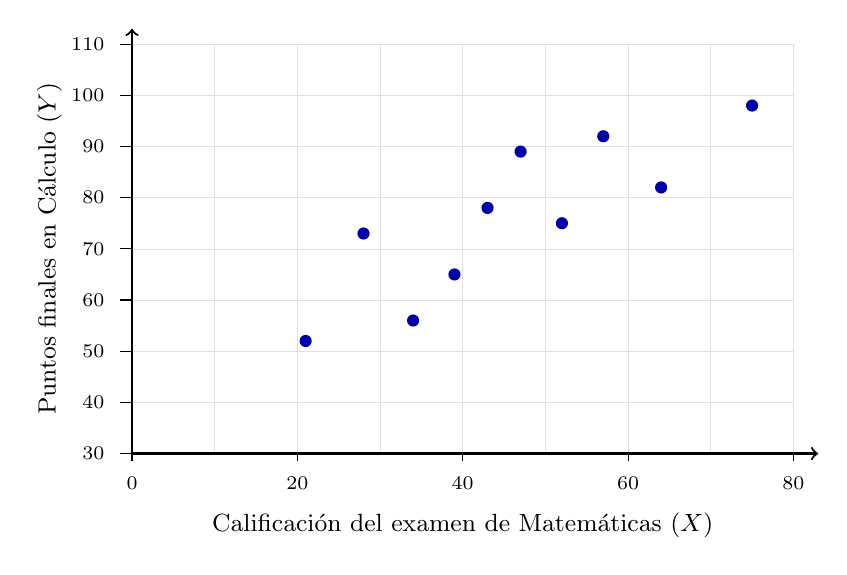
\begin{tikzpicture}[x=0.105cm,y=0.065cm]
    \draw[step=10,gray!25,very thin] (0,30) grid (80,110);
    \draw[->,thick] (0,30) -- (83,30);
    \draw[->,thick] (0,30) -- (0,113);
    \foreach \x in {0,20,40,60,80} {
        \draw (\x,30) -- (\x,28.5);
        \node[below=2pt,font=\scriptsize] at (\x,28.5) {\x};
    }
    \foreach \y in {30,40,50,60,70,80,90,100,110} {
        \draw (0,\y) -- (-1.5,\y);
        \node[left=2pt,font=\scriptsize] at (-1.5,\y) {\y};
    }
    \node[below=15pt,font=\small] at (40,28.5) {Calificación del examen de Matemáticas ($X$)};
    \node[rotate=90,font=\small] at (-10,70) {Puntos finales en Cálculo ($Y$)};
    \foreach \x/\y in {39/65,43/78,21/52,64/82,57/92,47/89,28/73,75/98,34/56,52/75} {
        \fill[blue!65!black] (\x,\y) circle (2.2pt);
    }
\end{tikzpicture}
\caption{Diagrama de dispersión de las calificaciones de Matemáticas y Cálculo.}
\label{fig:dispersion-calificaciones}
\end{figure}

En estos datos se aprecia una tendencia creciente: en general, estudiantes con calificaciones más altas en el examen de Matemáticas también obtuvieron más puntos en Cálculo. Sin embargo, los puntos no siguen un patrón perfectamente exacto. El gráfico sirve como primera descripción visual de la asociación; por sí solo no determina una ecuación predictiva ni cuantifica su precisión.
